\begin{activity}\label{A:0.1.1}
The graph of a function f is shown below. 

\begin{center}
    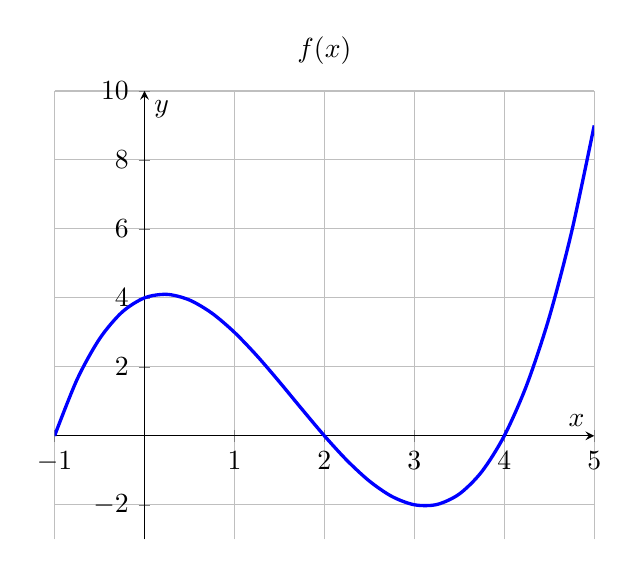
\begin{tikzpicture}
        \begin{axis}[axis lines=center, xmin=-1, xmax=5, ymin=-3, ymax=10, grid,
            xlabel={$x$}, ylabel={$y$}, title={$f(x)$}]
            \addplot[smooth, blue, very thick, domain=-1:5] {0.5*(x+1)*(x-2)*(x-4)};
        \end{axis}
    \end{tikzpicture}
\end{center}

\ba
\item What are the domain and range of $f$?
\item What are  $f(-1)$, $f(1)$, $f(3)$, $f(5)$?
\ea

\end{activity}\aftera
